\section{Results and Analysis}
\label{sec:results}

\subsection{Physical accounting exposes the strict disadvantage}

\begin{table*}[t]
  \caption{Verified selected-tensor endpoints at target ratio 0.258.
  Scope: \VerifiedModel{}, six MLP linear tensors, one seed, and
  \VerifiedEvalTokens{} held-out tokens.  ``Natural'' precedes final tail
  padding; ``Final'' is the complete research artifact whose stream offsets
  use 64-byte alignment.  Lower
  $\Delta$NLL/$\Delta$PPL is better.}
  \label{tab:exact-rate}
  \centering
  \begin{tabular}{lrrrrr}
\toprule
Endpoint & Natural B & Final B & $\Delta$NLL & $\Delta$PPL & norm. $H$ \\
\midrule
Q & 3,167,552 & 3,167,552 & +0.1982 & +15.644 & 0.01008 \\
Q + block scale & 3,250,496 & 3,250,496 & +0.1238 & +9.404 & 0.00577 \\
Q+S & 3,260,546 & 3,260,546 & +0.1224 & +9.293 & 0.00680 \\
Q+S (OBS) & 3,260,546 & 3,260,546 & +0.0956 & +7.156 & 0.00586 \\
\textbf{Q+L} & \textbf{3,248,832} & \textbf{3,248,832} & \textbf{+0.0905} & \textbf{+6.762} & \textbf{0.00463} \\
Q+S+L, strict & 3,233,152 & 3,248,832 & +0.0977 & +7.320 & 0.00507 \\
Q+S+L, +5{,}056 B & 3,253,888 & 3,253,888 & +0.0869 & +6.476 & 0.00457 \\
\bottomrule
\end{tabular}

\end{table*}

\cref{tab:exact-rate} gives selected bounded endpoints; the complete native
method set is retained in the released CSV.  Q+L and strict component-scaled
QSL are both \QLBytes{} bytes, but strict component-scaled QSL is
\StrictQSLMinusQLPPL{} perplexity worse.  Its natural file is
\StrictQSLNaturalBytes{} bytes and receives \StrictQSLTailPaddingBytes{} bytes
of tail padding to match the \QLNaturalBytes{}-byte Q+L file.  The control is
therefore a feasible but under-filled, per-layer-guarded candidate rather than
a budget-exhausted global frontier.  Equal padded length prevents an overrun;
it does not prove optimal use of the available natural bytes.  The relaxed QSL endpoint
adds only \RelaxedQSLExtraBytes{} bytes and is
\RelaxedQSLMinusQLPPL{} perplexity relative to Q+L, but its paired interval
crosses zero.  This is evidence of a discrete threshold, not a confirmed
frontier improvement.

\begin{figure*}[t]
  \centering
  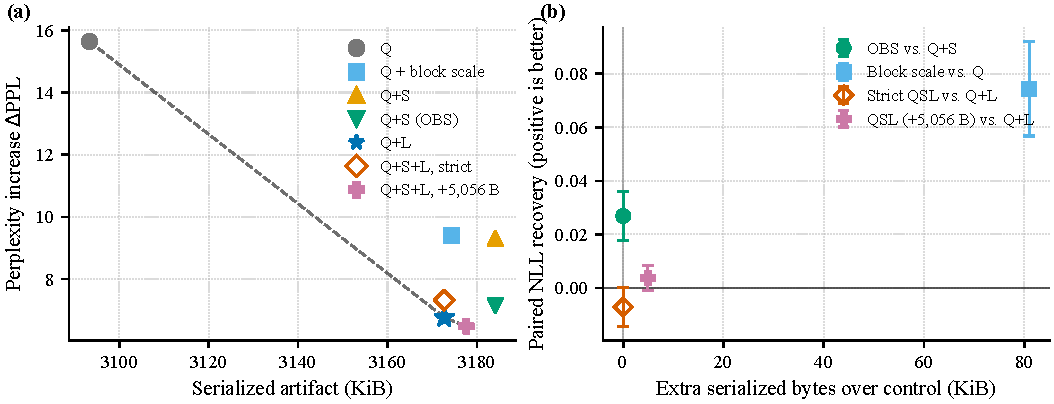
\includegraphics[width=0.98\textwidth]{figures/exact_rate_tradeoffs.pdf}
  \caption{Verified exact-rate trade-offs from committed CSV artifacts.
  (a) Physical bytes versus perplexity increase; only measured artifact files
  are plotted.  (b) Paired held-out NLL recovery and byte overhead for targeted
  repairs.  Error bars are descriptive normal intervals over 16 fixed windows,
  not population confidence intervals.  Scope is one seed and six selected
  Pythia-70M MLP tensors.}
  \label{fig:tradeoff}
\end{figure*}

\subsection{Which small parameters are used effectively?}

\begin{table}[t]
  \caption{Paired repair effects in the same bounded run.  Positive recovery
  favors the left method.  Intervals are descriptive over fixed windows.}
  \label{tab:repairs}
  \centering
  \resizebox{\columnwidth}{!}{\begin{tabular}{lrrrr}
\toprule
Comparison & $\Delta$ bytes & NLL recovery & 95\% interval & Wins \\
\midrule
OBS vs. Q+S & +0 & +0.0269 & [+0.0176, +0.0361] & 16/16 \\
Block scale vs. Q & +82,944 & +0.0744 & [+0.0568, +0.0921] & 16/16 \\
Strict QSL vs. Q+L & +0 & -0.0071 & [-0.0144, +0.0001] & 4/16 \\
QSL (+5{,}056 B) vs. Q+L & +5,056 & +0.0037 & [-0.0010, +0.0083] & 10/16 \\
\bottomrule
\end{tabular}
}
\end{table}

OBS is the clearest parameter-utilization result
(\cref{tab:repairs,fig:tradeoff}): it recovers \OBSRecovery{} mean NLL on an
unchanged support/value payload and improves \OBSWins{} windows.  It therefore
spends computation to make already-stored sparse values satisfy a local
stationarity condition.  Block scales recover \BlockRecovery{} NLL on all
  windows, but require \BlockExtraBytes{} additional bytes.  Q+L recovers more
  NLL per added byte than block scales in this tensor shape; the measured
  low-rank direction fits this residual more effectively, but one run does not
  establish a causal architectural advantage.  The strict QSL exchange instead
removes useful rank/support capacity to pay discrete sparse metadata and the
legacy per-layer alignment guard, and wins
only \StrictQSLWins{} windows against Q+L.

This suggests an analogue of scale protection for pruning: freeze a small
support, then optimize its values (OBS) rather than buying more survivors.
More generally, a repair is attractive when it changes existing stored state,
spans a high-energy residual direction, and avoids a new descriptor or index
threshold.

\subsection{Near-orthogonality is not sufficient}

At the strict endpoint,
$\rho_H(S,L)=\StrictSLRho{}$, but
$\rho_H(Q,S)=\StrictQSRho{}$ and
$\rho_H(Q,L)=\StrictQLRho{}$ (\cref{fig:geometry}).  S and L are nearly
orthogonal to each other; both cancel part of Q.  The three-way perturbation is
not mutually orthogonal, and the small S--L cross term cannot compensate for
their self costs or the capacity sacrificed to fit strict bytes.  This is the
observed counterpart of \cref{eq:exact-exchange}.

\begin{figure*}[t]
  \centering
  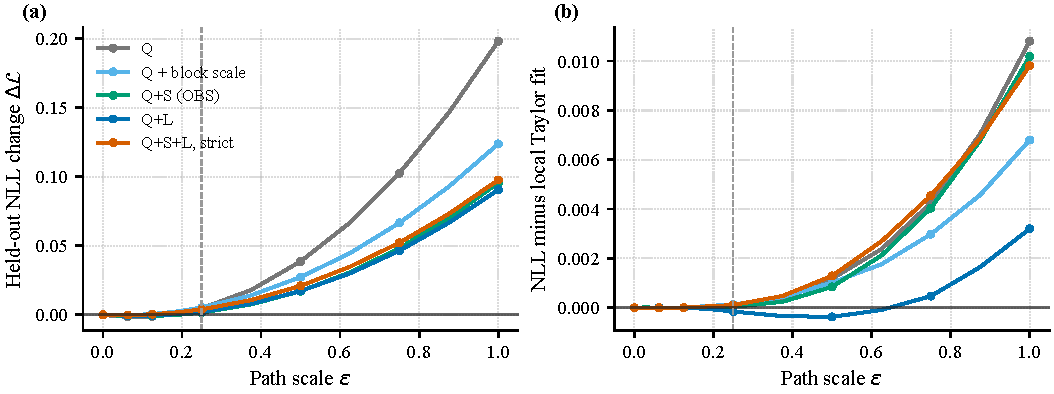
\includegraphics[width=0.98\textwidth]{figures/loss_landscape.pdf}
  \caption{Held-out loss landscapes for six codec directions in the original
  bounded probe.  Left: NLL along the 13-point interpolation.  Right: residual
  after the local linear--quadratic fit.  Proxy/path correlations range from
  \ProxyCorrMin{} to \ProxyCorrMax{}, yet nonzero linear terms and endpoint
  residuals require final NLL evaluation.  Scope is one seed, six selected
  Pythia-70M MLP tensors, and \VerifiedEvalTokens{} held-out tokens.}
  \label{fig:landscape}
\end{figure*}

The activation-Gram proxy tracks these particular paths closely
(\cref{fig:landscape}), but every fitted linear coefficient is negative.
Consequently, comparing only $\delta^\top H\delta$ omits a measurable
first-order contribution.  High correlation supports radial quadratic shape
only along each already selected direction; it does not validate cross-candidate
ranking and is not a certificate outside those directions or across models.

\subsection{Three scalability-smoke observations}

\begin{table*}[t]
\centering
\caption{Single-seed scalability smoke at target selected-weight artifact ratio 0.258. Pythia covers all MLP projections, while OPT and Qwen use ten depth-stratified MLP projections. Bytes are complete aligned research-codec files for selected tensors, not whole-model or production payloads. ``Strict$-$QL'' is the signed held-out NLL difference after tail padding to identical final bytes; the strict natural files leave 31,360/640/1,024 bytes unused for Pythia/OPT/Qwen. Negative favors the composite. Rows are not pooled or ranked across models.}
\label{tab:scaling-pilot}
\footnotesize
\setlength{\tabcolsep}{4.5pt}
\begin{tabular*}{\textwidth}{@{\extracolsep{\fill}}lrrrrrrr@{}}
\toprule
Model / scope & \shortstack{Tensors /\\M params} & \shortstack{QL=strict\\bytes (rate)} & $\Delta$NLL QL & $\Delta$NLL strict & Strict$-$QL & $\rho_{SL}$ & $\rho_{QS}/\rho_{QL}$ \\
\midrule
Pythia-70M / full MLP & 12 / 12.58 & 6,497,344 (0.2581) & +0.1963 & +0.2017 & +0.0054 & +0.026 & -0.334/-0.588 \\
OPT-125M / 5-depth MLP & 10 / 23.59 & 12,158,976 (0.2577) & +0.0735 & +0.0744 & +0.0009 & +0.087 & -0.367/-0.611 \\
Qwen3-0.6B / 5-depth MLP & 10 / 31.46 & 16,196,352 (0.2574) & +0.0226 & +0.0299 & +0.0073 & +0.022 & -0.521/-0.743 \\
\bottomrule
\end{tabular*}
\end{table*}


\begin{figure*}[t]
  \centering
  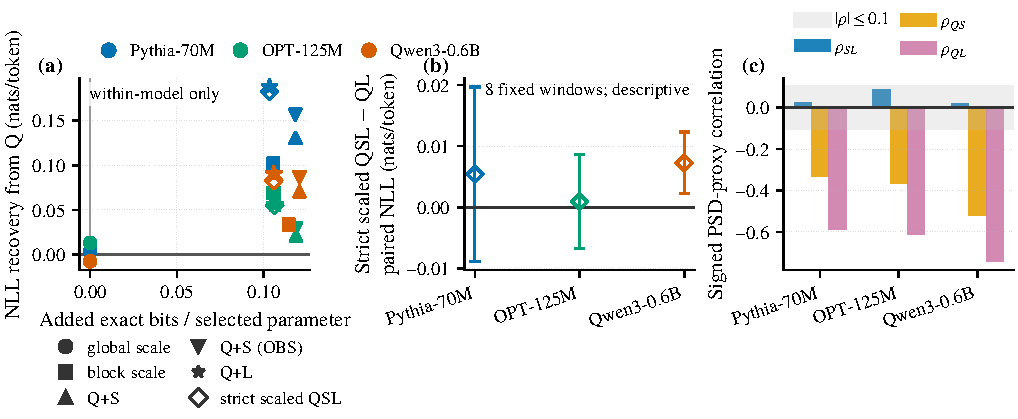
\includegraphics[width=0.99\textwidth]{figures/scaling_pilot_efficiency_geometry.pdf}
  \caption{Mechanism behavior in three separate seed-\ScalePilotSeed{}
  scalability-smoke jobs.  (a) Within each color/model, held-out NLL recovery
  from Q versus added exact file bits per selected parameter; the zero-byte
  scale point is direct folded re-estimation, not infinite efficiency.
  (b) Conservative strict component-scaled QSL minus Q+L after tail padding
  to identical final file bytes; the strict natural files underfill their Q+L
  caps by 31,360, 640, and 1,024 bytes for Pythia, OPT, and Qwen, respectively;
  error bars are descriptive mean $\pm1.96$ sample standard errors over eight
  fixed windows, not confidence intervals or significance tests.  (c) Signed
  activation-Gram correlations; the band marks $|\rho|\le0.1$, while negative
  Q--S/Q--L values denote cancellation.  Tokenizers and tensor scopes differ,
  so magnitudes are not ranked across models and rates are not whole-model
  compression ratios.}
  \label{fig:scaling-smoke}
\end{figure*}

The strict scaled composite is higher-NLL than Q+L in all three decoded,
final-byte-equal but naturally underfilled endpoints: by
\ScalePilotPythiaStrictMinusQLNLL{} on Pythia,
\ScalePilotOPTStrictMinusQLNLL{} on OPT, and
\ScalePilotQwenStrictMinusQLNLL{} on Qwen.  The fixed-window descriptive
interval crosses zero for Pythia and OPT; Qwen favors Q+L in seven of eight
windows and its interval remains positive.  At the same time,
$\rho_H(S,L)$ is \ScalePilotPythiaStrictSLRho{},
\ScalePilotOPTStrictSLRho{}, and \ScalePilotQwenStrictSLRho{}, respectively,
whereas every Q--S and Q--L correlation is negative
(\cref{tab:scaling-pilot,fig:scaling-smoke}).  Thus the coherence diagnostic
remains compatible with local S--L additivity, but the realized exchange
condition in \cref{eq:exact-exchange} fails for each tested conservative
endpoint.  Because unused natural bytes were not reallocated across layers,
these observations do not reject every budget-exhausted composite.

The parameter-utilization controls are more mechanism-specific.  Block scales
improve Q in every job while paying positive descriptor/scale bytes, and OBS
value re-estimation improves Q+S in all three without changing the sparse file.
Folded global-scale re-estimation helps Pythia and OPT but hurts Qwen at the
same bytes.  This is precisely why zero-byte state reuse is attractive yet
still requires held-out endpoint validation: low parameter cost does not imply
a universally beneficial update.  The committed CSVs contain all 33 endpoints
and 234 path points.  The appendix tabulates every endpoint and visualizes the
78 Q+L/strict path points in
\cref{tab:scaling-pilot-all-endpoints,fig:scaling-paths}; none is collapsed
into a cross-model mean.

\subsection{What would establish a combination advantage?}

None of the current tail-padded strict candidates does relative to Q+L; OPT also contains
a lower-NLL, slightly smaller Q+block-scale endpoint.  A convincing positive
result at the same
compression rate must (i) use an identical tensor manifest and actual bytes,
(ii) keep each component's self cost in its low-curvature regime, (iii) control
all signed cross terms without calling cancellation orthogonality, (iv) clear
the discrete rank/support/descriptor threshold, and (v) retain a positive
held-out endpoint gain after the byte exchange.  In the notation of
\cref{eq:exact-exchange}, these requirements reduce to an executable
$G_A(r)>P_A(u)+\Gamma_A(u,r)$ test.  The new global allocator and large-model
method-ablation matrix are designed to test that inequality while allowing Q,
Q+S$_{\rm OBS}$, and Q+L as nested degenerate states.  Until those jobs
complete, they remain planned and are not silently promoted to results.
